\documentclass[11pt,a4paper]{article}

% ---------------------------------------------------------------------------
% GovGuide -- Final Technical Report (AgenTriX 2026, Team 24)
% Compile:  latexmk -pdf report.tex      (or run pdflatex twice)
% Figures live in ./figures (ASCII-named copies of the originals).
% ---------------------------------------------------------------------------

\usepackage[T1]{fontenc}
\usepackage[utf8]{inputenc}
\usepackage{lmodern}
\usepackage[a4paper,margin=2.4cm]{geometry}
\usepackage{microtype}
\usepackage{graphicx}
\usepackage{xcolor}
\usepackage{booktabs}
\usepackage{tabularx}
\usepackage{longtable}
\usepackage{xltabular}
\usepackage{array}
\usepackage{enumitem}
\usepackage{float}
\usepackage{caption}
\usepackage{amssymb}
\usepackage{listings}
\usepackage{fancyhdr}
\usepackage[colorlinks=true,linkcolor=blue!45!black,urlcolor=blue!55!black,citecolor=blue!45!black]{hyperref}

\graphicspath{{figures/}}

\definecolor{accent}{HTML}{1F6FEB}
\definecolor{codebg}{HTML}{F6F8FA}
\definecolor{codeframe}{HTML}{D0D7DE}

\newcolumntype{Y}{>{\raggedright\arraybackslash}X}
\newcommand{\done}{\textcolor{green!55!black}{\checkmark}}
\newcommand{\tableitem}[1]{\texttt{#1}}

\lstdefinestyle{code}{
  basicstyle=\ttfamily\footnotesize,
  breaklines=true,
  columns=fullflexible,
  keepspaces=true,
  showstringspaces=false,
  frame=single,
  framesep=5pt,
  rulecolor=\color{codeframe},
  backgroundcolor=\color{codebg},
  xleftmargin=4pt,
}
\lstset{style=code}

\captionsetup{font=small,labelfont=bf}

% Absorb the few unbreakable \texttt{} runs in prose so nothing bleeds into the margin.
\emergencystretch=3em

\pagestyle{fancy}
\fancyhf{}
\fancyhead[L]{\small GovGuide --- Final Technical Report}
\fancyhead[R]{\small AgenTriX 2026 \textbullet{} Team 24}
\fancyfoot[C]{\thepage}
\renewcommand{\headrulewidth}{0.4pt}

% ===========================================================================
\begin{document}

% --------------------------- Title page -----------------------------------
\begin{titlepage}
  \centering
  \vspace*{1.6cm}
  {\Huge\bfseries GovGuide\par}
  \vspace{0.5cm}
  {\Large An Agentic AI Navigator for Sri Lankan\\[2pt] Government \& Citizen Services\par}
  \vspace{1.0cm}
  {\large\itshape Final Technical Report\par}
  \vspace{2.0cm}

  \begin{tabular}{rl}
    \textbf{Team}     & Team 24 \\[3pt]
    \textbf{Domain}   & Government \& Citizen Services, Sri Lanka \\[3pt]
    \textbf{Scope}    & English-only MVP (Sinhala/Tamil on the roadmap) \\
  \end{tabular}

  \vfill
  {\large A hierarchical multi-agent system (LangGraph) over a\\
   self-expanding, citation-grounded RAG knowledge base,\\
   delivered behind a FastAPI + SSE backend in a hexagonal architecture.\par}
  \vspace{1.2cm}
  {\small June 2026\par}
\end{titlepage}

% --------------------------- Abstract -------------------------------------
\thispagestyle{fancy}
\section*{Abstract}
Accessing a government service in Sri Lanka suffers from deep \emph{information asymmetry}:
the exact documents, fees, correct office and processing sequence are known mainly to counter
staff, change over time, vary by district, and are rarely consolidated online. The result is the
familiar \emph{3--4 repeated failed visits}, whose cost falls hardest on rural and low-literacy
citizens. \textbf{GovGuide} is an agentic AI navigator that takes a plain-language request,
identifies the correct service, runs a minimal clarifying interview to pin the exact case
(branch + district), retrieves the current requirements with a \emph{cited, dated source for every
fact}, and produces a printable \emph{Action Pack} (document checklist, fees, the right office, and
the step sequence).

Its core innovation is a \textbf{self-expanding RAG} knowledge base: because the government domain
is too large to pre-index, a corrective-retrieval grader detects knowledge gaps and an autonomous
acquisition team researches, curates and writes the missing knowledge back to the store --- so the
first user's research is cached for everyone after. Trust is protected by grounding, provenance, a
human moderation gate, and a \emph{confidence-gated serving} rule that refuses to answer rather than
mislead. This report documents the problem, the architecture (a justified hybrid of styles realised
in a strict hexagonal, ports-and-adapters codebase), the data model, the ten-agent workflow, the
technology stack, the as-built implementation (delivered in verifiable stages with 132 automated
tests passing under strict typing and linting), the API contract, a full security/cryptography
threat model, and the results against the AgenTriX rubric.

\tableofcontents
\clearpage

% ======================================================================
\section{Introduction}
\label{sec:intro}

\subsection{Problem statement}
For any Sri Lankan government service --- land deed transfer, NIC renewal, business registration,
birth-certificate correction, passports --- the precise set of required documents, the fees, the
authorised office and officer, and the order of steps are effectively tacit knowledge held at the
counter. These requirements \textbf{change over time}, \textbf{vary by district}, and are
\textbf{almost never consolidated} in one current place online; official sites are incomplete or
outdated. Citizens therefore make repeated failed trips, each time discovering one more missing
document. There is no single, current, plain-language, \emph{personalised} source that tells a
citizen exactly what to do for \emph{their} specific case.

\subsection{Why naive solutions fail}
\begin{itemize}[leftmargin=1.4em]
  \item \textbf{The domain is huge.} Hundreds of services across many departments --- a knowledge
        base cannot be fully built up front, and it goes stale.
  \item \textbf{Processes branch.} Land transfer differs for \emph{inheritance vs.\ sale vs.\ gift};
        requirements differ by \emph{district}. A generic answer is wrong for the individual.
  \item \textbf{Trust matters.} A confidently wrong answer about a government process wastes a real,
        paid trip. Answers must be grounded and attributable.
\end{itemize}

\subsection{Chosen domain}
Government \& Citizen Services, Sri Lanka. The system focuses on flagship services chosen to showcase
both hero features --- the branching clarifying interview and the self-expanding RAG:
\textbf{Land Deed Transfer} (the best showcase of the branching interview) and \textbf{NIC services}
(high volume, relatable). Services not yet present in the knowledge base are handled on demand by the
acquisition loop rather than being pre-built.

% ======================================================================
\section{Solution Overview}
\label{sec:solution}

A citizen describes their need in plain language; GovGuide then:
\begin{enumerate}[leftmargin=1.6em]
  \item \textbf{Identifies the correct service} from the natural-language request.
  \item Runs a short \textbf{clarifying interview} --- asking only the questions needed to pin the
        exact sub-case (branch + district).
  \item \textbf{Retrieves current requirements} (documents, fees, office + officer, timeline) from a
        curated knowledge base, \emph{with a cited source and \texttt{last\_verified} date} for every
        fact.
  \item \textbf{If the knowledge base has a gap}, autonomous agents \textbf{research, curate, and
        write the answer back} (the self-expanding RAG loop), then answer.
  \item Generates a \textbf{personalised, printable Action Pack}: the exact document checklist for
        their case, total estimated cost, the step-by-step office sequence, and the right office.
  \item \textbf{Self-improves} --- after a visit, citizens submit a short experience report that,
        after moderation, updates the knowledge base.
\end{enumerate}

\paragraph{Value \& commercial model.} B2G licensing to ICTA/government as a citizen-facing
front-end over existing portals (cuts counter congestion and repeat visits); a B2C freemium tier
(free guidance, premium document-prep / appointment booking); and an anonymised
service-bottleneck data product for policy makers. The defensible moat is the
\emph{self-expanding, crowd-verified knowledge base} that improves with every query and report.

% ======================================================================
\section{Requirements \& Quality Attributes}
\label{sec:requirements}

\subsection{Functional requirements}
\begin{center}
\begin{tabularx}{\linewidth}{@{}l Y l@{}}
\toprule
\textbf{ID} & \textbf{Requirement} & \textbf{Use case} \\
\midrule
FR-1 & Accept a free-text English service request & UC1 \\
FR-2 & Ask minimal clarifying questions to select a variant + district & UC2, UC7 \\
FR-3 & Return grounded, cited requirements / fees / office / timeline & UC3, UC8 \\
FR-4 & Detect insufficient knowledge and acquire it autonomously & UC9--UC11 \\
FR-5 & Produce a printable Action Pack & UC4 \\
FR-6 & Accept and queue citizen experience reports & UC6, UC13 \\
FR-7 & Let a moderator promote \texttt{auto\_gathered} $\to$ \texttt{verified} & UC12, UC13 \\
\bottomrule
\end{tabularx}
\end{center}

\subsection{Quality attributes (the architecture drivers)}
Architecture is the set of decisions that are hard to change later; each earns its place by serving
a quality attribute, never ``because it is cool''.

\begin{center}
\begin{tabularx}{\linewidth}{@{}l l Y@{}}
\toprule
\textbf{\#} & \textbf{Quality attribute} & \textbf{How the architecture responds} \\
\midrule
QA-1 & Trustworthiness \emph{(dominant)} & Grounded RAG; every fact carries \texttt{source\_id} +
\texttt{last\_verified}; corrective-RAG grader (A5); confidence-gated serving (A6); moderation (B4). \\
QA-2 & Responsiveness & Local embeddings (no API round-trip); cheap two-stage grader; SSE streaming of
agent-step progress; local-source-pool-first research. \\
QA-3 & Cost / free-tier survivability & Bounded acquisition loops ($N\le2$); merged calls; local
embeddings; a central rate-limited LLM gateway; query$\to$answer cache. \\
QA-4 & Modifiability & Ports \& adapters (hexagonal); Strategy + Adapter patterns. \\
QA-5 & Extensibility of knowledge & Self-expanding RAG --- lazy, on-demand ingestion. \\
QA-6 & Availability / graceful degradation & Local source pool primary, web fallback; loop-cap
$\to$ graceful fallback (``contact this office directly''). \\
QA-7 & Security \& privacy & \texttt{*.gov.lk} allow-list; moderation gate; minimal PII; schema-validated
outputs. \\
QA-8 & Traceability / observability & One typed \texttt{GraphState} + \texttt{SqliteSaver} checkpointer;
correlation ids; optional LangSmith traces. \\
\bottomrule
\end{tabularx}
\end{center}

\noindent\textbf{Priority ranking (on conflict):} QA-1 Trustworthiness $>$ QA-6 Availability $>$
QA-2 Responsiveness $>$ QA-3 Cost $>$ QA-4/5 evolvability. Concretely, we would rather \emph{refuse
to answer} than answer fast or answer at all --- which is exactly why low-confidence
\texttt{auto\_gathered} facts trigger the fallback instead of an Action Pack.

% ======================================================================
\section{Use Cases}
\label{sec:usecases}

The actors are the \textbf{Citizen} (primary), the \textbf{Moderator/Admin}, and two external system
actors: the \textbf{LLM provider} (Gemini) and the \textbf{Web / Source Pool}. Figure~\ref{fig:usecase}
shows the use-case model.

\begin{figure}[ht]
  \centering
  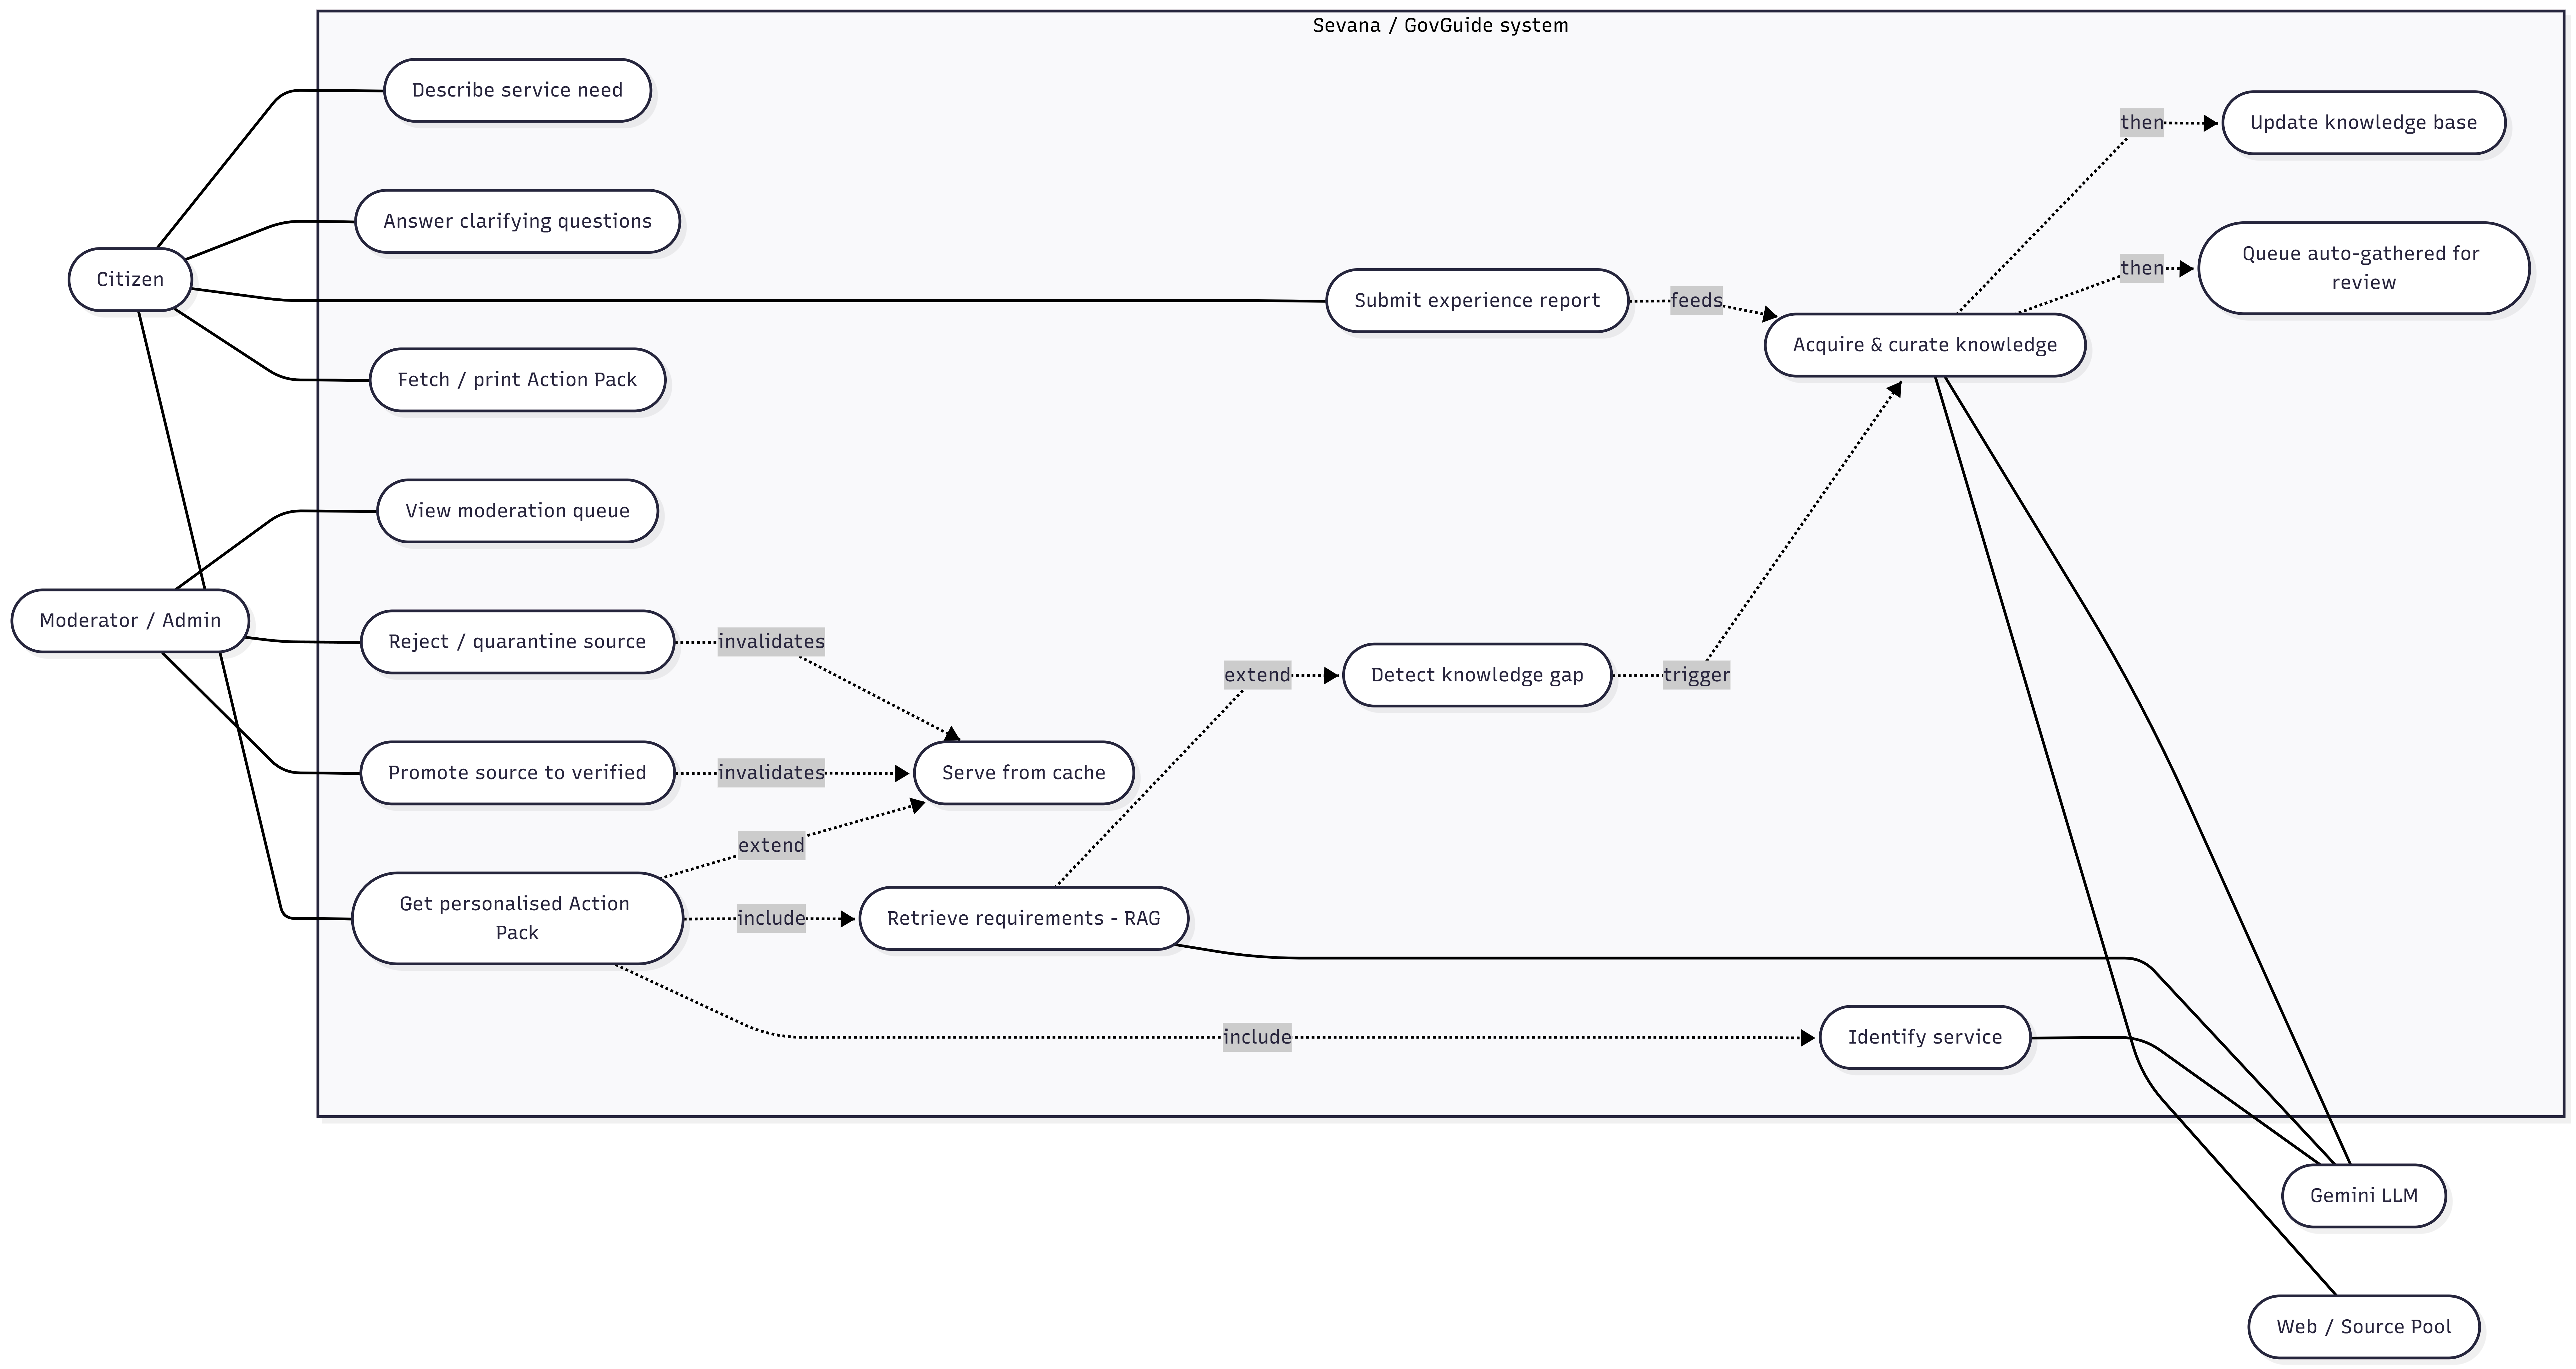
\includegraphics[width=\linewidth,height=0.62\textheight,keepaspectratio]{use-case-diagram}
  \caption{Use-case diagram. The citizen-facing cases (describe need, answer clarifications, get and
  print the Action Pack, find the office, submit an experience report) \emph{include} service
  identification and RAG retrieval, which \emph{extends} into gap detection and autonomous knowledge
  acquisition; the moderator reviews and approves auto-gathered knowledge and experience reports.}
  \label{fig:usecase}
\end{figure}

\paragraph{Key scenarios (also the demo script).}
\begin{description}[leftmargin=0pt,style=nextline]
  \item[Scenario A --- Seeded service, branching (happy path).] ``I inherited my father's land and
  want to transfer the deed.'' A1/A2 identify \emph{Land Deed Transfer}; A3 asks only
  \emph{inheritance/sale/gift?} and \emph{which district?}; A4/A5 find sufficient seeded knowledge;
  A6 returns a cited Action Pack as printable output.
  \item[Scenario B --- Unseen service (the self-expanding RAG showcase).] ``How do I register a
  business name as a sole proprietor?'' A4 retrieves little; A5 grades \texttt{GAP}; B1--B3 research,
  curate and write the knowledge back; the loop re-retrieves and A6 answers, labelled
  ``newly gathered, pending verification''. The knowledge base has grown live.
  \item[Scenario C --- Feedback loop.] A returning citizen reports ``they also asked for a Grama
  Niladhari letter.'' The report enters the same B2$\to$B3 pipeline as \texttt{pending}; a moderator
  verifies it, and future citizens see it automatically.
\end{description}

% ======================================================================
\section{Architecture}
\label{sec:architecture}

\subsection{A justified hybrid of styles}
No single style fits the whole system, so each part uses the style that best serves its dominant
driver. Naming them makes the design defensible.

\begin{center}
\begin{tabularx}{\linewidth}{@{}l Y@{}}
\toprule
\textbf{Style} & \textbf{Where it is used / driver} \\
\midrule
Orchestration (Supervisor) & Control flow across agents (the LangGraph supervisor) --- correctness,
traceability (QA-1, QA-8). \\
Blackboard / Data-centred & The shared \texttt{GraphState} every agent reads/writes --- traceability. \\
Pipe-and-Filter & The acquisition pipeline B1$\to$B2$\to$B3 --- extensibility (QA-5). \\
Layered (Hexagonal) & API $\to$ application $\to$ adapters $\to$ data --- modifiability, security. \\
Repository / Data-centred & The knowledge base (Chroma + SQLite) and the source pool --- correctness,
availability. \\
\bottomrule
\end{tabularx}
\end{center}

\noindent It is \textbf{orchestrated, not event-driven} --- there is no message bus; the supervisor
decides every hop. That is a deliberate single-node design choice.

\subsection{C4 Level 1--2: Context and Containers}
Figure~\ref{fig:containers} shows the system in context and its deployable containers. The citizen's
critical path (browse $\to$ ask $\to$ answer) is \textbf{synchronous}; progress during the slow
gap-fill is pushed to the UI over \textbf{Server-Sent Events (SSE)} so the wait is always visible.

\begin{figure}[ht]
  \centering
  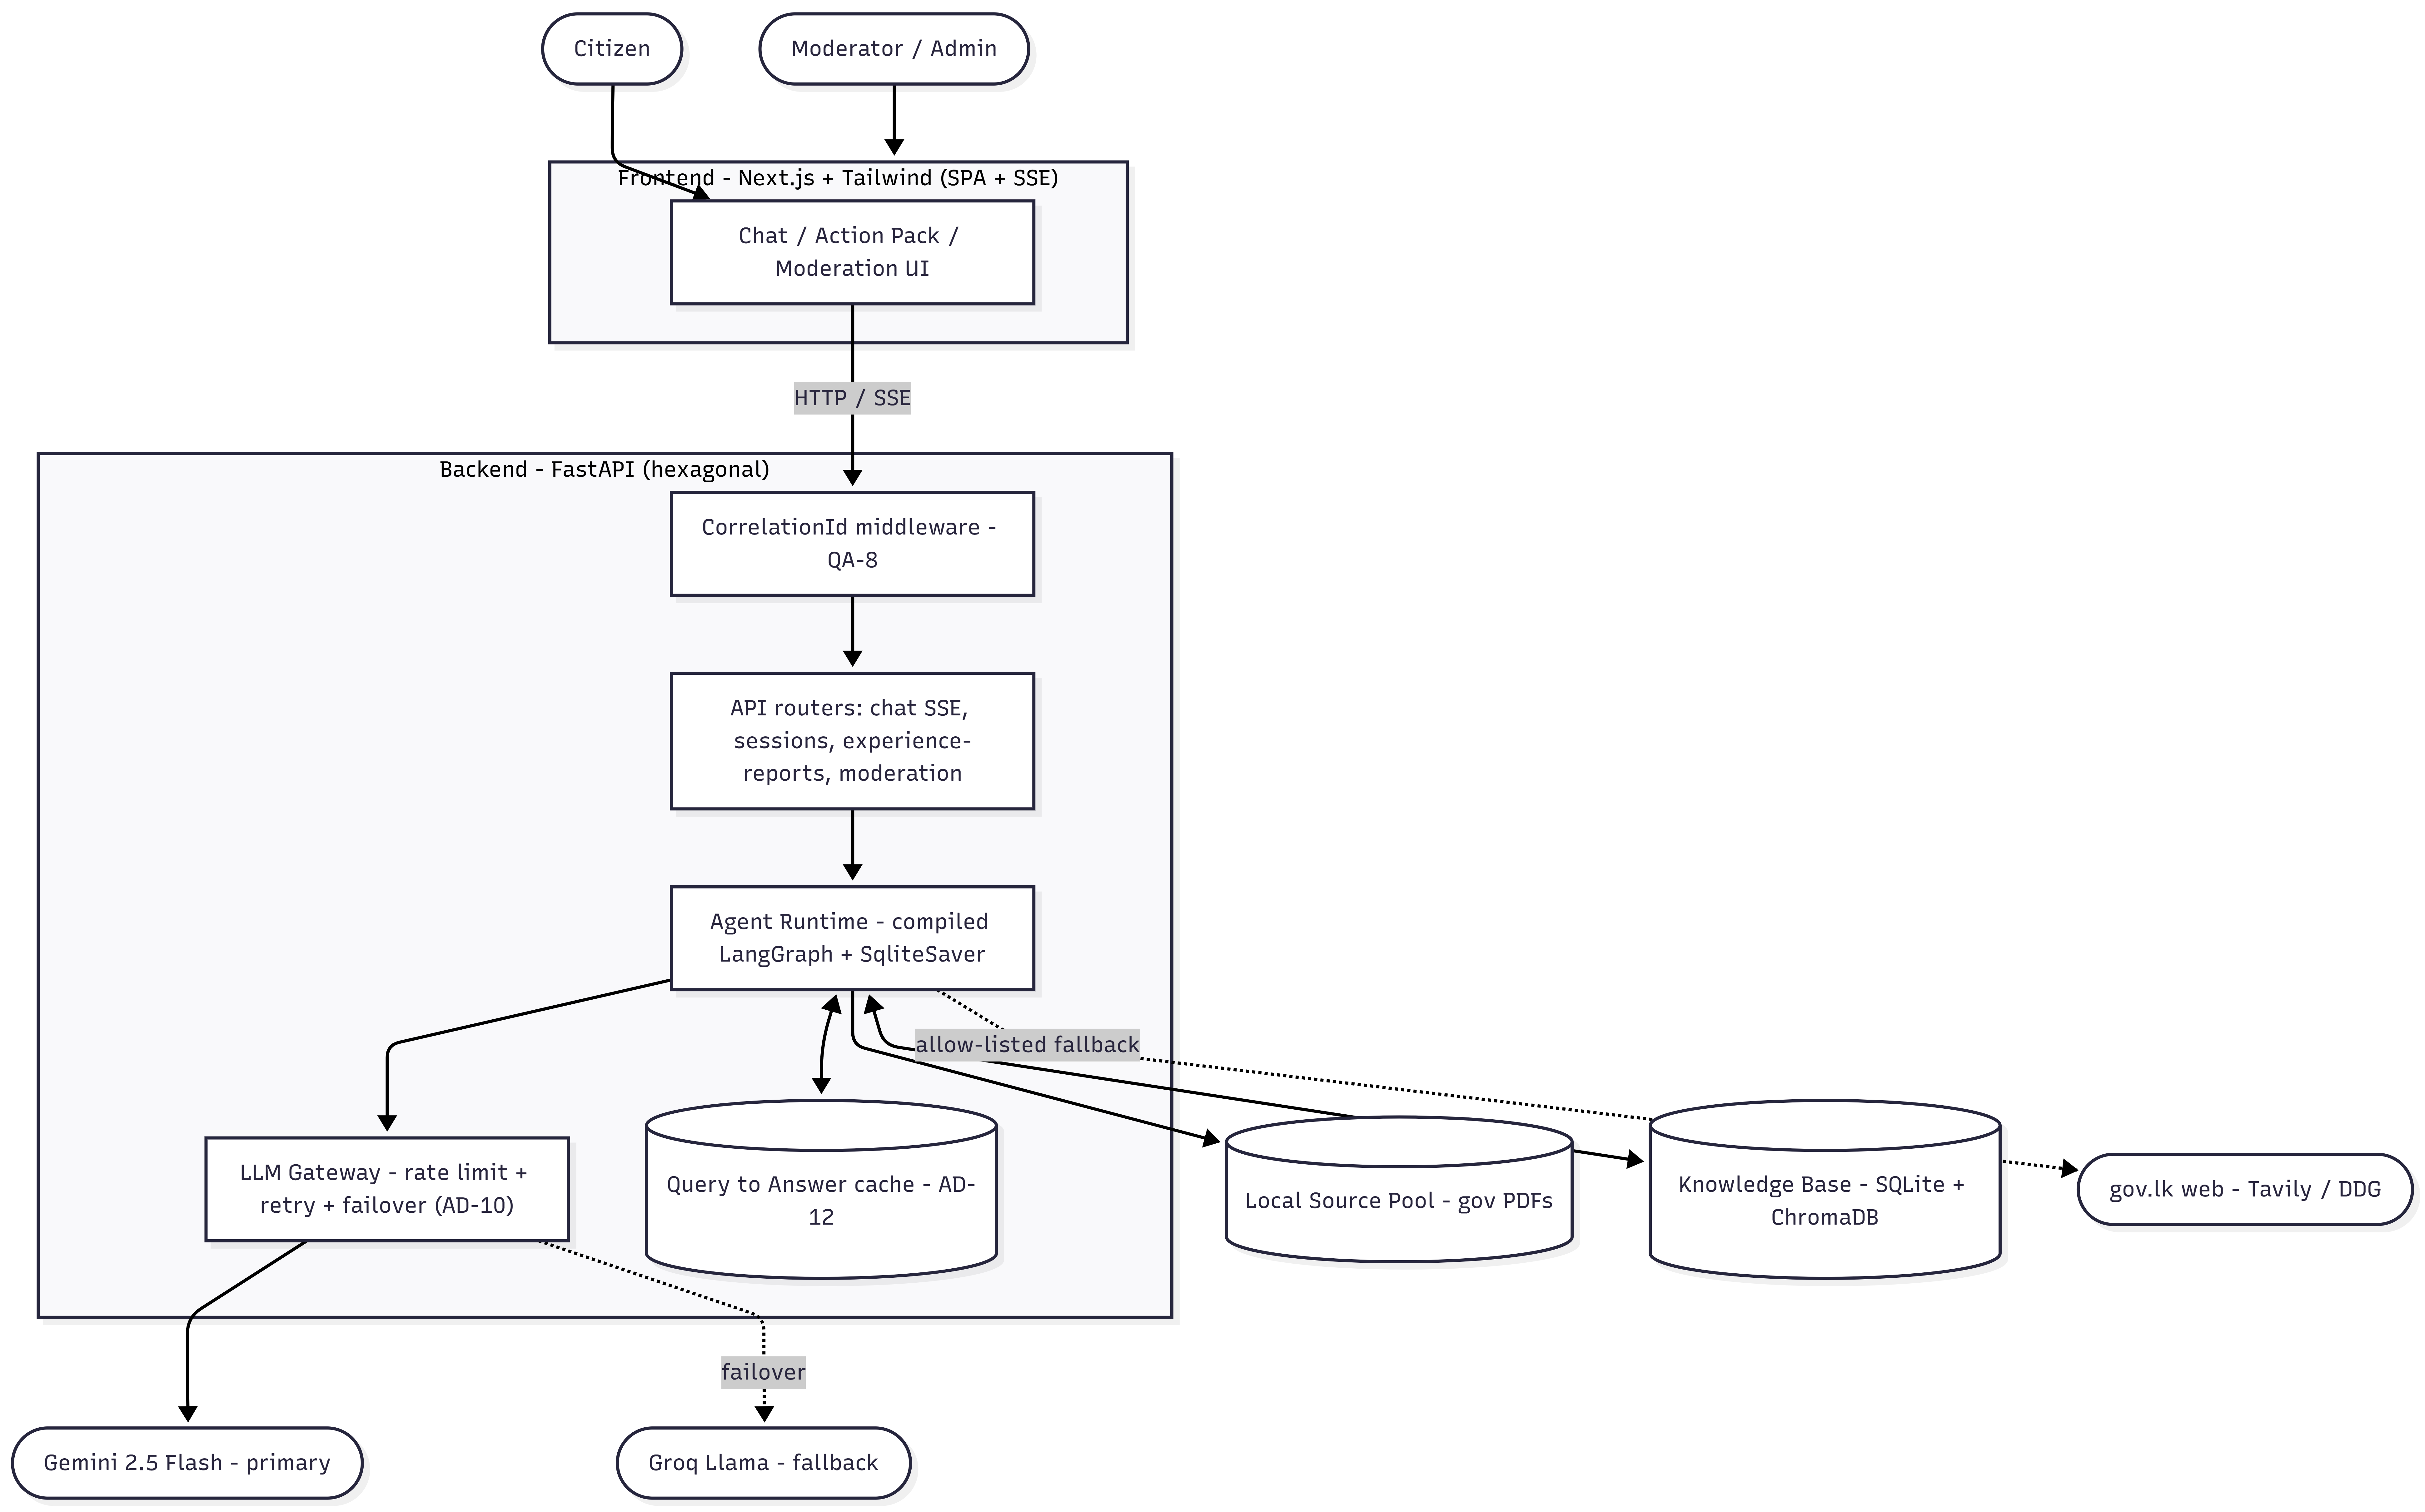
\includegraphics[width=\linewidth,keepaspectratio]{system-context-containers}
  \caption{C4 context + container view. A Next.js + Tailwind SPA talks to a FastAPI backend over
  HTTP/SSE; the backend invokes the LangGraph agent runtime, which calls Gemini through a
  rate-limited LLM gateway, reads/writes the Chroma + SQLite knowledge base, searches a local source
  pool first and live \texttt{*.gov.lk} web as fallback, and short-circuits repeats through a
  query$\to$answer cache.}
  \label{fig:containers}
\end{figure}

\subsection{Hexagonal layering (ports \& adapters)}
The backend is laid out so that \textbf{dependencies point inward} (Figure~\ref{fig:hexagonal}):
\texttt{domain} imports nothing; \texttt{application} (use cases / agents) imports only
\texttt{domain.ports}; \texttt{adapters} implement those ports; \texttt{api} wires the concrete
adapters in at startup. Swapping a provider (Gemini$\to$Groq, Chroma$\to$pgvector) touches only
\texttt{adapters/}. This makes the modifiability claim (QA-4) \emph{structural}, not aspirational ---
and it is enforced automatically by a test that AST-scans the domain package and fails the build on
any framework import.

\begin{figure}[ht]
  \centering
  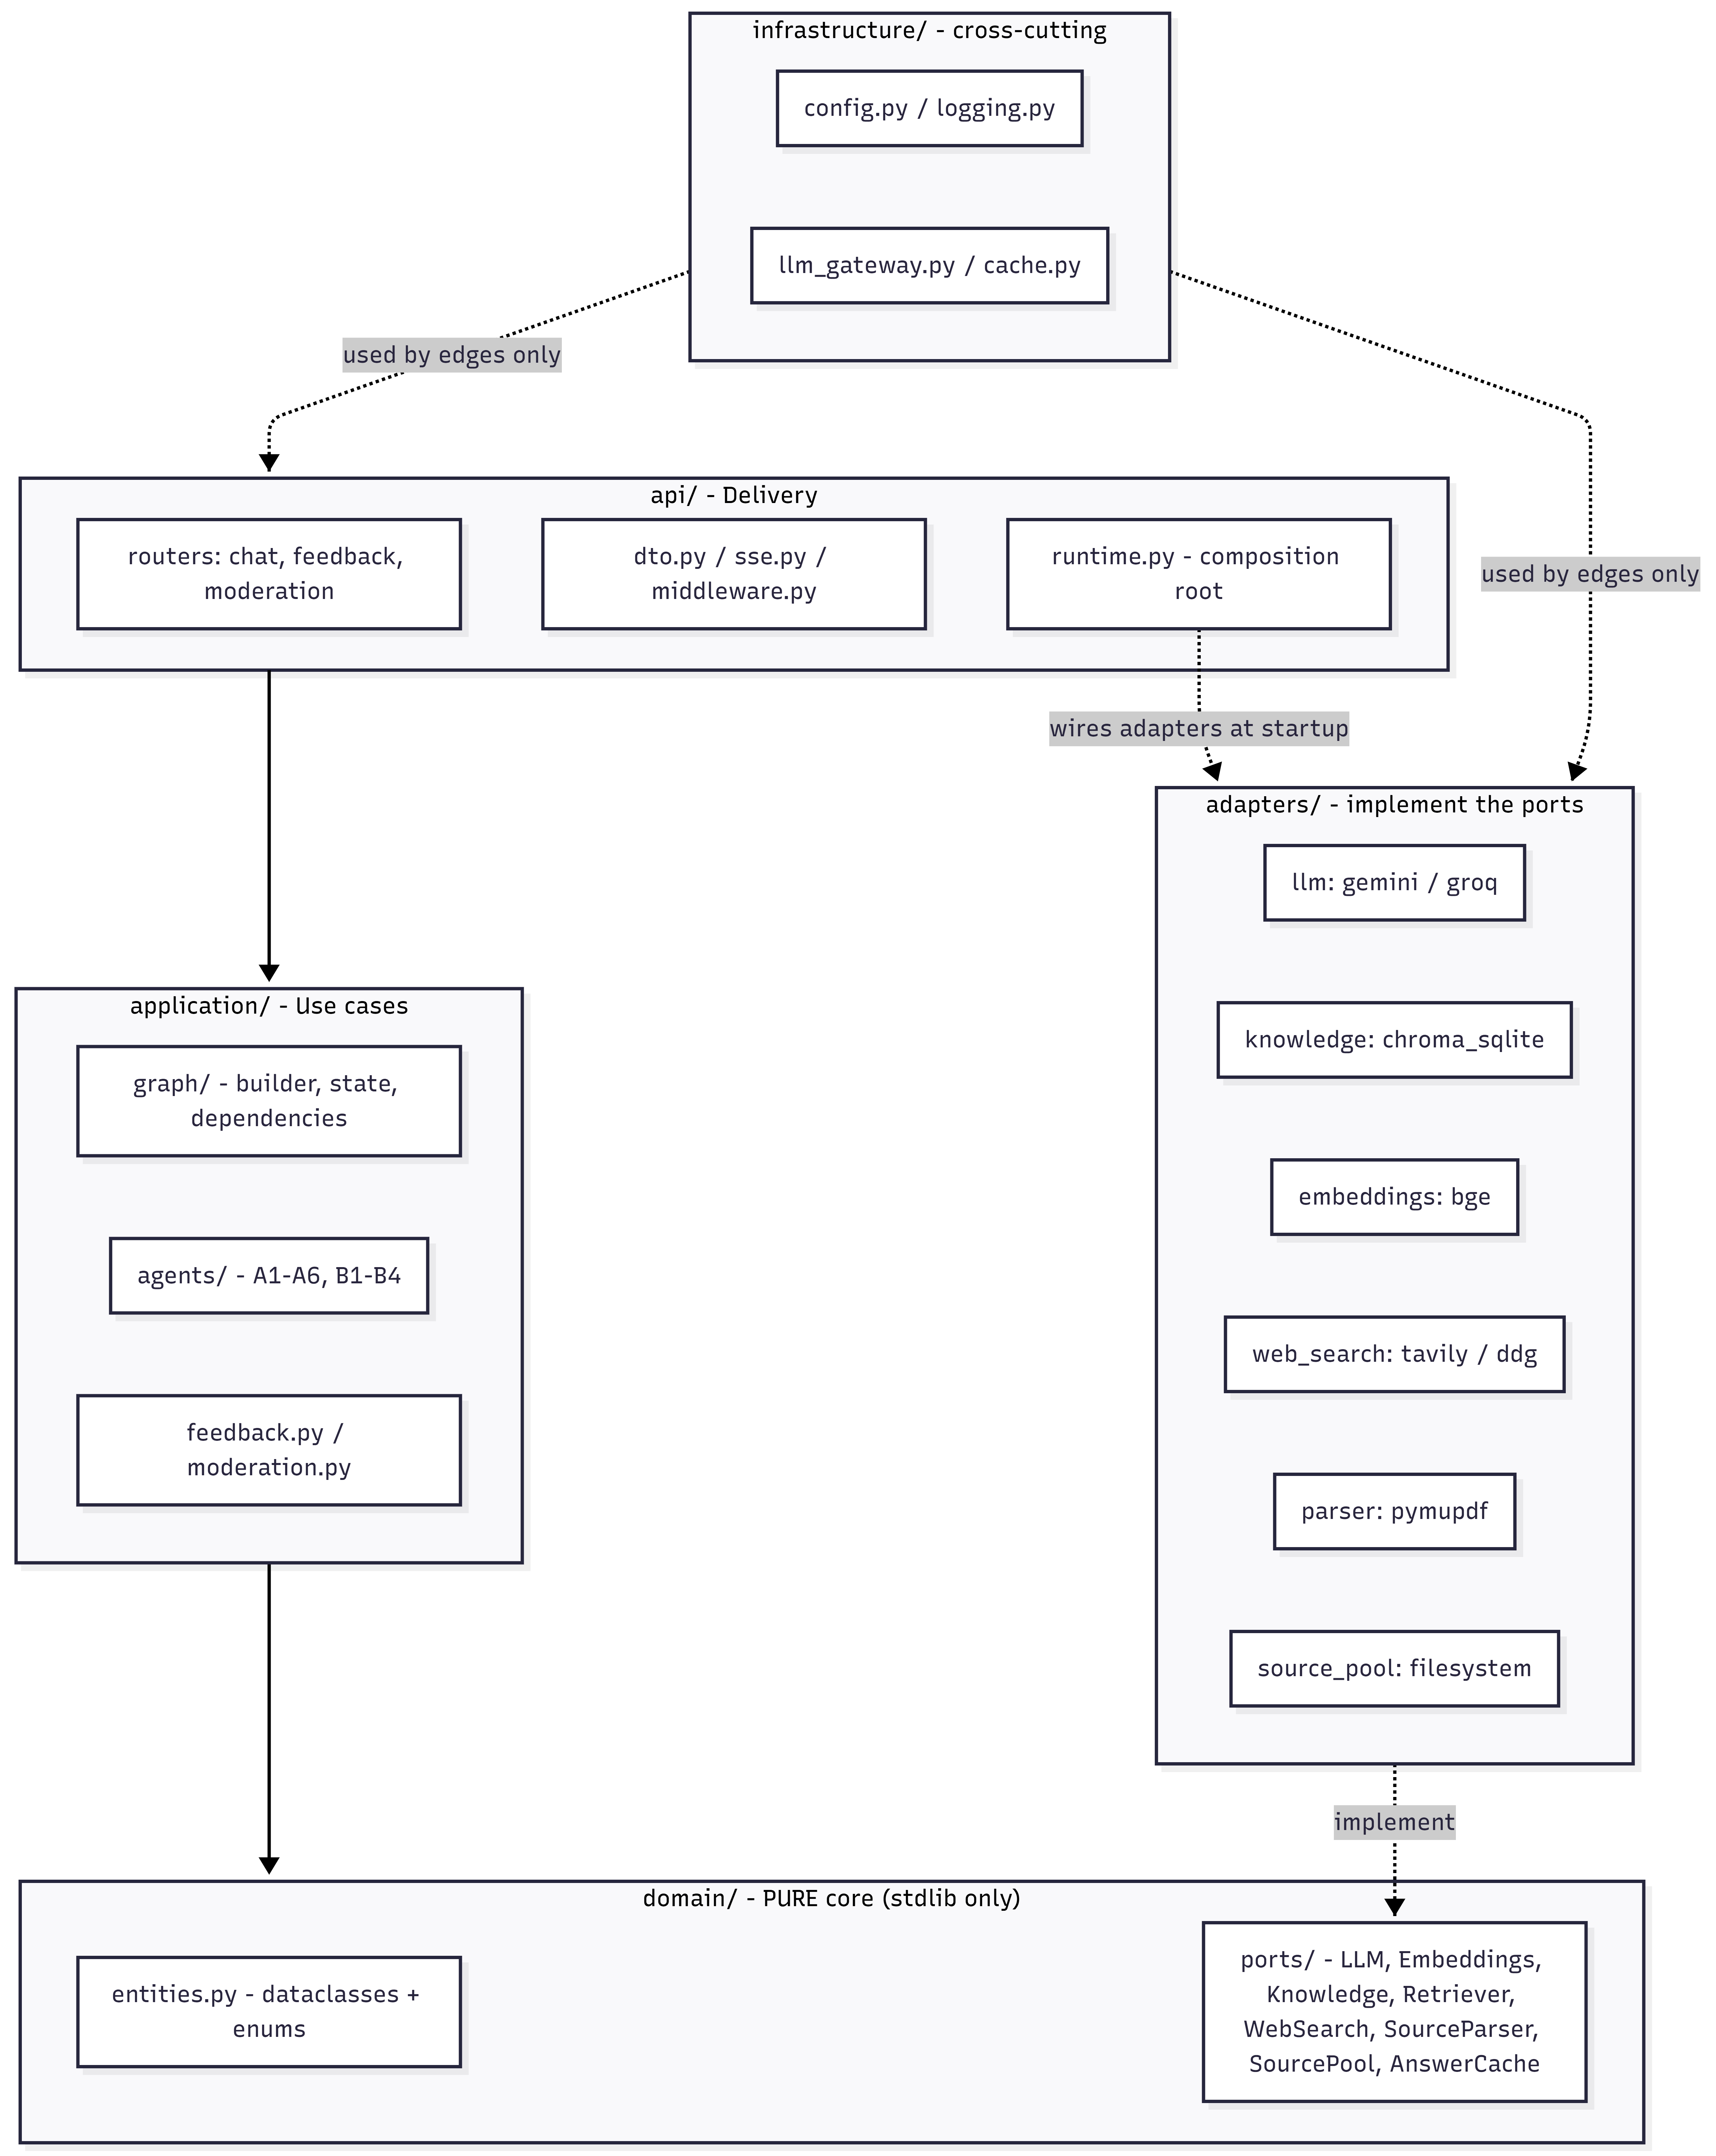
\includegraphics[width=\linewidth,keepaspectratio]{hexagonal-layers}
  \caption{Hexagonal layers and the dependency rule. The pure domain core (entities + port
  interfaces) sits at the centre; application use cases depend only on ports; adapters and the
  FastAPI delivery layer sit on the outside and are swappable.}
  \label{fig:hexagonal}
\end{figure}

\subsection{The agent runtime (C4 Level 3)}
Opening the agent-runtime container reveals the supervisor plus two teams
(Figure~\ref{fig:graph}): the synchronous \textbf{Answering} team (A1--A6) and the
\textbf{Knowledge-Acquisition} team (B1--B4), triggered only on a gap. The supervisor is realised as
\emph{state-driven conditional edges} (it spends zero LLM quota on routing), and the clarifying
interview is a real LangGraph \texttt{interrupt()} that pauses the run and resumes on the citizen's
reply.

\begin{figure}[ht]
  \centering
  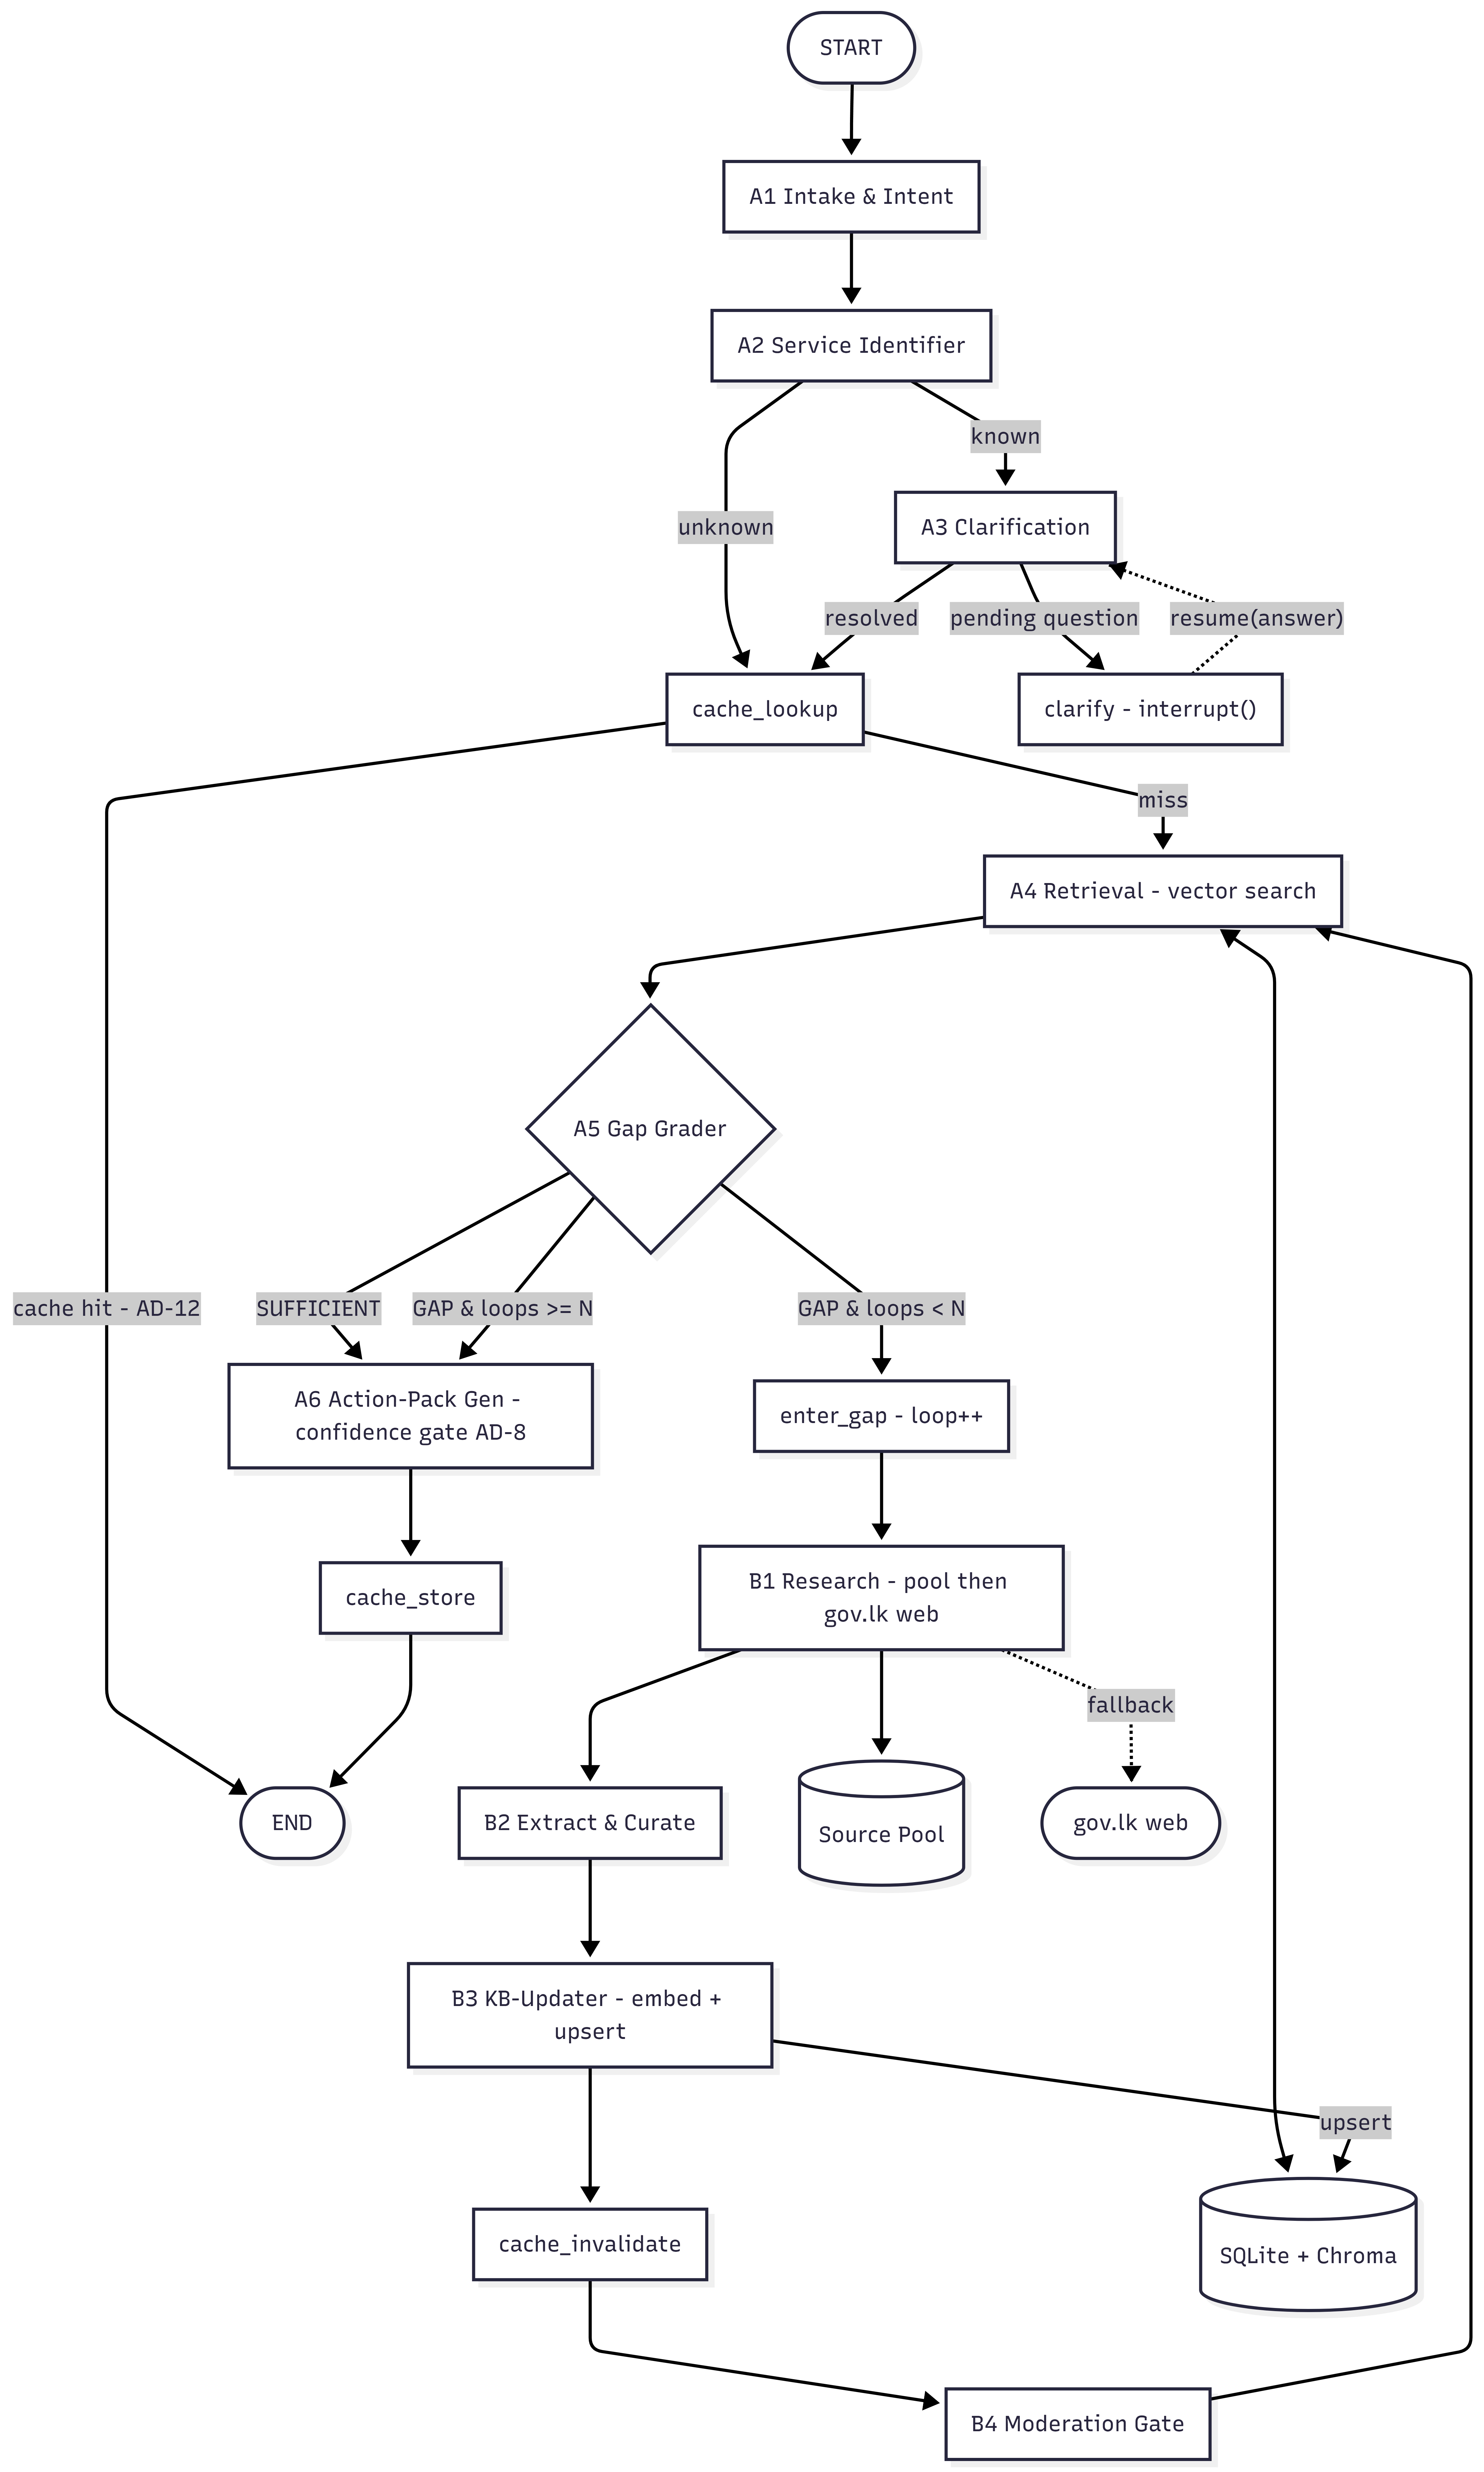
\includegraphics[width=\linewidth,height=0.78\textheight,keepaspectratio]{agent-graph}
  \caption{The compiled LangGraph. \texttt{START}$\to$A1$\to$A2; an unknown service routes straight
  to retrieval, a known service to the A3$\leftrightarrow$clarify interview, then A4 retrieval $\to$
  A5 grader. \texttt{SUFFICIENT}$\to$A6; \texttt{GAP} with \texttt{loops}$<N$ enters the bounded
  acquisition loop (\texttt{enter\_gap}$\to$B1$\to$B2$\to$B3$\to$B4$\to$A4); an exhausted loop falls
  through to A6 in fallback mode. Optional cache nodes short-circuit resolved repeats.}
  \label{fig:graph}
\end{figure}

\subsection{Design patterns applied}
\begin{center}
\begin{tabularx}{\linewidth}{@{}l Y@{}}
\toprule
\textbf{Pattern} & \textbf{Where} \\
\midrule
Strategy & \texttt{LLMProvider}, \texttt{WebSearch}, the A5 grader (threshold vs.\ LLM). \\
Adapter & Each external API (Gemini, Tavily, PyMuPDF) behind a common port. \\
Fa\c{c}ade & FastAPI calls one \texttt{graph} invocation over the whole multi-agent subsystem. \\
Repository & \texttt{KnowledgeStore} over SQLite + Chroma. \\
State / Blackboard & Supervisor routing over \texttt{GraphState} transitions. \\
Decorator & The LLM gateway \emph{is} an \texttt{LLMProvider} wrapping the real one (throttle/retry). \\
Pipe-and-Filter & The B1$\to$B2$\to$B3 acquisition pipeline. \\
\bottomrule
\end{tabularx}
\end{center}

\subsection{Architecture decision record (key, hard-to-reverse decisions)}
Each decision states its trade-off, because every architectural choice costs something.

{\footnotesize
\begin{xltabular}{\linewidth}{@{}p{0.9cm} Y Y@{}}
\toprule
\textbf{ID} & \textbf{Decision} & \textbf{Trade-off accepted} \\
\midrule
\endhead
AD-1 & Hierarchical supervisor + 2 teams (not single ReAct, not swarm) & More nodes to build/wire;
central control point. \\
AD-2 & Self-expanding RAG (corrective-RAG + lazy ingestion) & First-hit latency; auto-gathered facts
need confidence-gating + moderation. \\
AD-3 & Blackboard \texttt{GraphState} + \texttt{SqliteSaver} checkpointer & Shared mutable state can
bloat; heavy artifacts kept out of the persisted state (lean). \\
AD-4 & Local \texttt{bge-base-en-v1.5} embeddings & $\sim$440\,MB model + cold start; English-only;
must use the same model at write and read. \\
AD-5 & SQLite + ChromaDB (not Postgres + pgvector) & Single-writer concurrency limits; migrate to
Postgres post-event. \\
AD-6 & Gemini 2.x Flash (free tier) behind an \texttt{LLMProvider} port & Free-tier rate limits +
lock-in risk; mitigated by the port and AD-10. \\
AD-7 & Local source pool first, live web fallback & Pool must be pre-curated and can go stale;
allow-listing limits reach. \\
AD-8 & Confidence-gated serving of auto-gathered knowledge & May refuse a correct-but-low-confidence
find (under-answering beats misleading). \\
AD-9 & Hexagonal (ports \& adapters) layout & More indirection/boilerplate --- justified by
modifiability + testability. \\
AD-10 & Central rate-limited LLM gateway & A shared throughput bottleneck in front of the LLM. \\
AD-11 & Synchronous orchestration (no event bus) & No async fan-out / independent scaling. \\
AD-12 & Query$\to$answer cache keyed by service+variant+district & Risk of a stale answer ---
mitigated by invalidation on KB upsert / moderation. \\
\bottomrule
\end{xltabular}}

% ======================================================================
\section{The Self-Expanding RAG}
\label{sec:rag}

This is the core innovation, and it answers a hard constraint directly: \emph{we cannot pre-build a
knowledge base for the entire government domain, so the knowledge base must grow itself on demand.}
Academically this is \textbf{Corrective RAG (CRAG) + lazy / on-demand ingestion}.

\paragraph{The loop.}
\begin{enumerate}[leftmargin=1.6em]
  \item \textbf{Retrieve} (A4) --- query the existing KB (vector + structured).
  \item \textbf{Grade} (A5) --- judge whether the retrieved context actually answers the query:
        \texttt{SUFFICIENT} or \texttt{GAP}.
  \item On \textbf{GAP}: \textbf{B1 Research} (local source pool first, then allow-listed web)
        $\to$ \textbf{B2 Extract \& Curate} (raw text into schema-shaped records with provenance and
        a \texttt{retrieved\_date}) $\to$ \textbf{B3 KB-Updater} (dedup, chunk, embed locally, upsert
        into Chroma + SQLite, tagged \texttt{confidence} and
        \texttt{verification\_status = auto\_gathered}) $\to$ re-retrieve. The loop is \textbf{bounded
        by $N$} (default 2).
  \item The answer from newly-gathered knowledge is \textbf{labelled} ``newly gathered, pending
        verification'' with its sources, so trust stays honest.
\end{enumerate}

\paragraph{Why it beats the alternatives.} A static pre-built KB is never complete for a huge domain
and goes stale; web-search-on-every-query is slow, blows the free-tier rate limit, and never learns;
GraphRAG and fine-tuning are too heavy or paid for a free-tier build. The chosen design grows
the KB \emph{lazily, only where real users hit gaps}; the first user's research is cached for everyone
after --- fresh, free-tier-efficient, and a genuine data moat.

\paragraph{Guardrails.} \texttt{acquisition\_loops}$\le N$ prevents runaway loops/cost; the source
allow-list prevents ingesting junk; the moderation gate (B4) keeps auto-gathered knowledge usable but
provisional; dedup on upsert (by URL + SHA-256 content hash) avoids re-ingesting the same source. The
same B2$\to$B3 pipeline also ingests \textbf{citizen experience reports}, so the system improves from
real-world outcomes, not only web research.

% ======================================================================
\section{Data Model}
\label{sec:datamodel}

A relational schema in \textbf{SQLite} holds structured facts + provenance (the source of truth and
the basis of the ER diagram), mirrored into \textbf{ChromaDB} for vector retrieval. Structured records
make the Action Pack deterministic (exact fees, exact office) while the vector store powers fuzzy
natural-language retrieval; provenance lives on every record so answers can cite a dated source.
Figure~\ref{fig:er} shows the entity-relationship model.

\begin{figure}[ht]
  \centering
  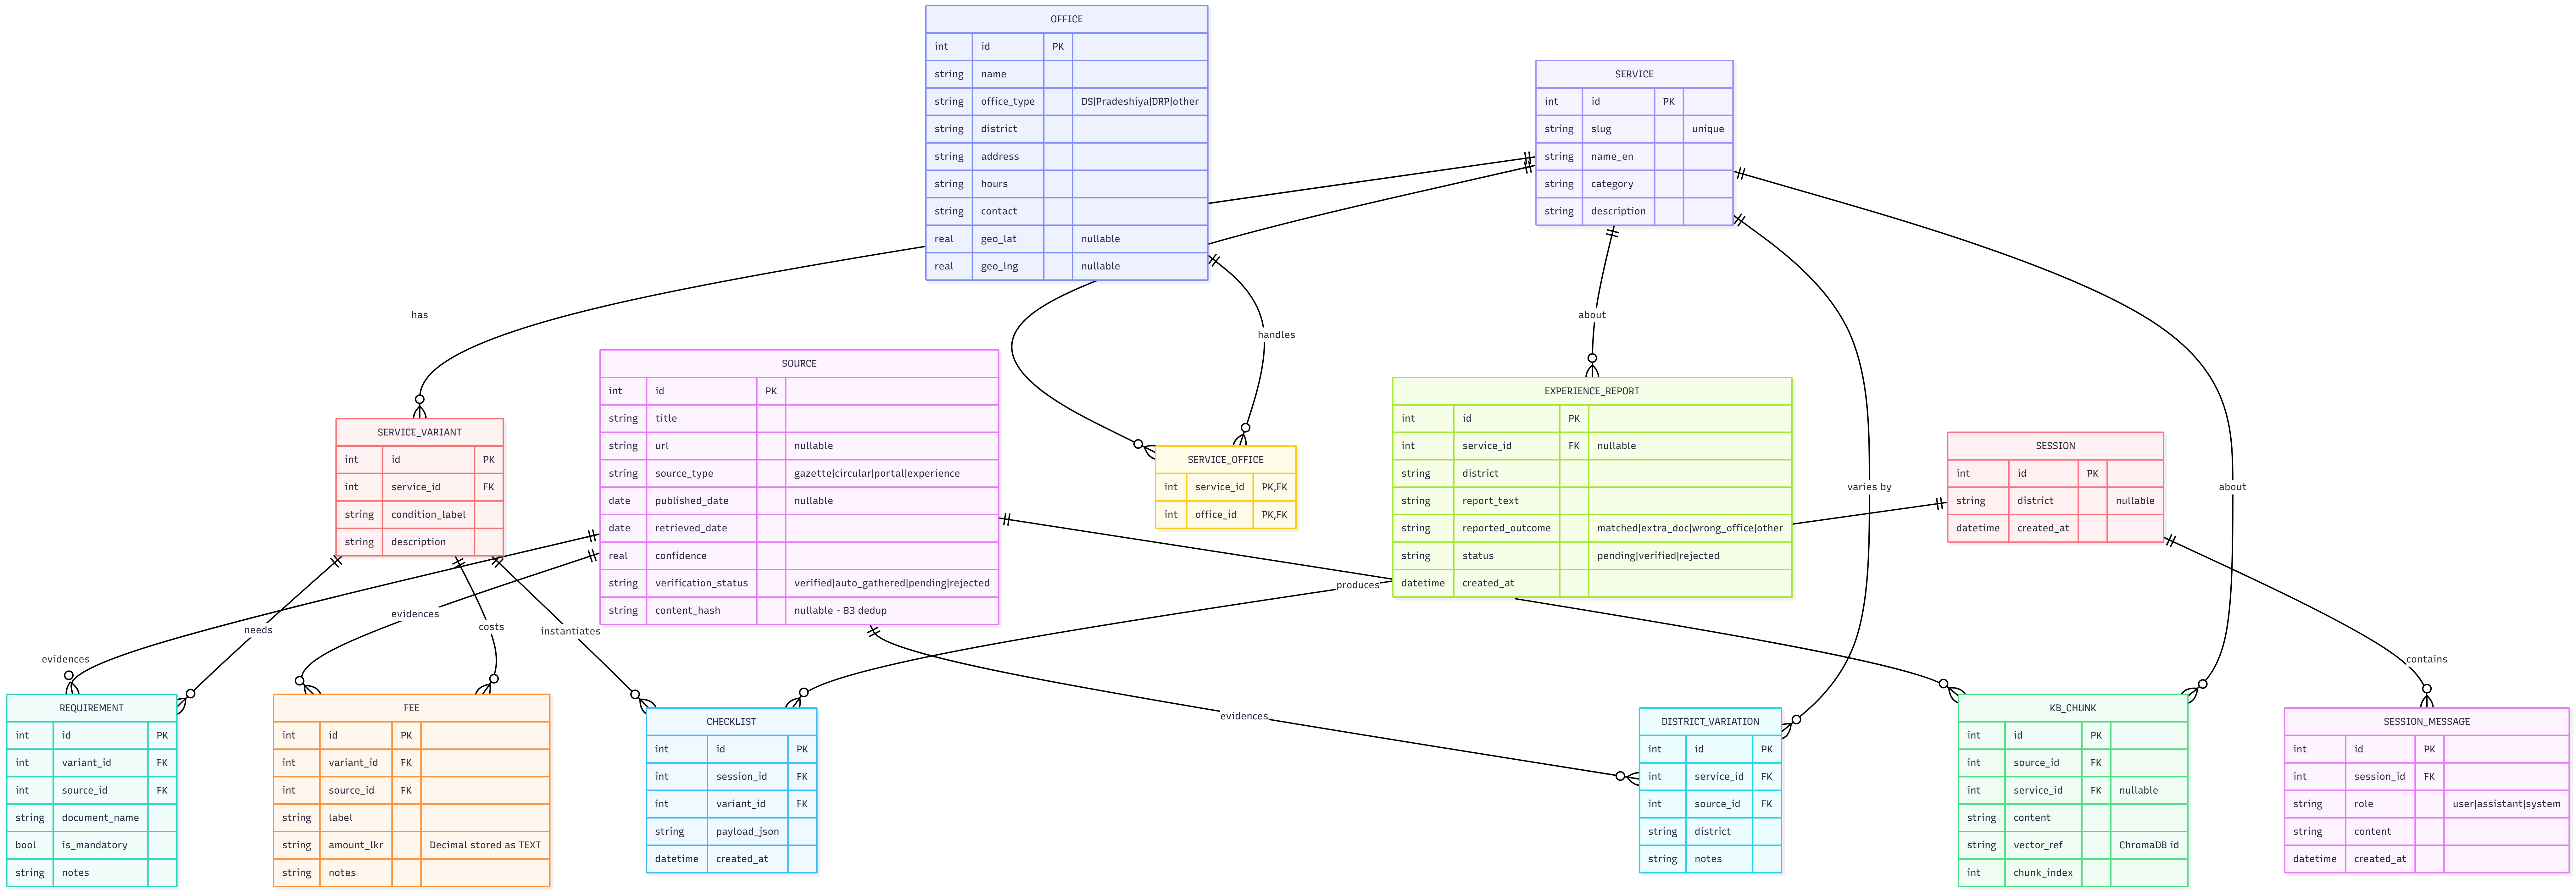
\includegraphics[width=\linewidth,height=0.80\textheight,keepaspectratio]{er-diagram}
  \caption{Entity-relationship model. A \texttt{SERVICE} has \texttt{SERVICE\_VARIANT}s,
  \texttt{DISTRICT\_VARIATION}s and \texttt{SERVICE\_OFFICE} links; a variant needs
  \texttt{REQUIREMENT}s and \texttt{FEE}s; every \texttt{SOURCE} evidences requirements/fees/variations
  and is chunked into \texttt{KB\_CHUNK}s (each linked to its Chroma vector). Sessions, messages,
  checklists and experience reports complete the runtime model.}
  \label{fig:er}
\end{figure}

\paragraph{The confidence serving gate.} A \texttt{SOURCE} carries two \emph{independent} trust
signals that must not be conflated: \texttt{verification\_status} decides the \emph{label} shown to the
citizen, while \texttt{confidence} (0--1) decides whether to \emph{answer at all}. Before A6 renders an
Action Pack from auto-gathered facts, the supporting facts' confidence is compared to a threshold
$\tau$ (default \textbf{0.6}). If \texttt{confidence}\,$\ge\tau$ the pack is rendered (labelled
``pending verification''); if \texttt{confidence}\,$<\tau$ it is \emph{not} rendered and the graceful
fallback is returned. \texttt{verified} facts bypass the gate. A \emph{label} does not stop a
\emph{bad} answer --- this gate does.

\paragraph{As-built deltas (code vs.\ ER).} The pure-domain dataclasses mirror the ER with a few
intentional, logged differences. The \texttt{OFFICE.type} column becomes \texttt{office\_type} in
code (it would otherwise shadow the Python \texttt{type} builtin). The SQLite schema adds a
\texttt{content\_hash} column on \texttt{source} for B3 dedup, and stores money as text to preserve
decimal precision. \texttt{VerificationStatus} gains a fourth value, \texttt{rejected}, so a
moderator's reject is a real quarantine --- de-indexed, but the row is kept so dedup still blocks
re-ingestion. The domain also adds runtime value objects that are not tables: \texttt{RetrievedChunk}
(the A4 output) and the \texttt{ActionPack} family (the A6 output).

% ======================================================================
\section{Agent Design}
\label{sec:agents}

The system is a \textbf{hierarchical multi-agent} design: one supervisor coordinates two teams. We
stop deliberately at two levels (supervisor $\to$ team $\to$ worker) --- no supervisor-of-supervisors.
Each agent has a single responsibility, which keeps every node small, independently testable, and
individually explainable.

\subsection{Team 1 --- Answering (A1--A6)}
\begin{center}
\begin{tabularx}{\linewidth}{@{}l l Y@{}}
\toprule
\textbf{ID} & \textbf{Agent} & \textbf{Responsibility (as built)} \\
\midrule
A1 & Intake \& Intent & One structured LLM call: normalise the request into intent + entities; seed
slots from stated entities. \\
A2 & Service Identifier & Retrieval-assisted classification: lexical catalog match + a short LLM
disambiguation when candidates are close; no confident match $\to$ \texttt{service\_unknown} (gap
path). \\
A3 & Clarification & Minimal slot-filling interview as a LangGraph \texttt{interrupt()}; pins
\texttt{variant\_id} + district, asks one grounded question at a time, caps the interview and defaults
to the common variant when exhausted. \\
A4 & Retrieval (RAG) & Local query embedding + vector search filtered by service; writes only chunk
text + provenance to state (leanness). \\
A5 & Gap Grader & Two-stage corrective-RAG switch: a cheap score/coverage threshold first, a short LLM
check only on the borderline band; emits \texttt{grade} + \texttt{answer\_confidence}; biases to
\texttt{GAP} when unsure. \\
A6 & Action-Pack Generator & Confidence gate \emph{first} (AD-8); assembles documents/fees/office
\emph{deterministically from the store}; the LLM is constrained to sequencing the \texttt{steps} only;
attaches citations + \texttt{last\_verified} and the verification label. \\
\bottomrule
\end{tabularx}
\end{center}

\noindent An important free-tier optimisation: only \textbf{A1} strictly needs the LLM; A2/A3/A5/A6
take an \emph{optional} provider with deterministic fallbacks, so the answering path is quota-light and
the LLM is spent only where it adds value (intent, disambiguation, phrasing, borderline grading, step
narration).

\subsection{Team 2 --- Knowledge Acquisition (B1--B4)}
\begin{center}
\begin{tabularx}{\linewidth}{@{}l l Y@{}}
\toprule
\textbf{ID} & \textbf{Agent} & \textbf{Responsibility (as built)} \\
\midrule
B1 & Research & Pure port-orchestrator: search the \texttt{SourcePool} (local-first) then
allow-listed \texttt{WebSearch}; write raw candidates to \texttt{acquisition\_buffer}. \\
B2 & Extract \& Curate & One structured LLM call per doc into a fixed schema + a \texttt{SOURCE}
(\texttt{auto\_gathered}); \texttt{confidence = authority(origin) $\times$ extraction\_certainty};
drops docs with no identifiable service. \\
B3 & KB-Updater & Idempotent: dedup by URL + SHA-256; reuse-or-create service/variant (never
overwriting \texttt{verified}); chunk $\to$ embed locally $\to$ upsert vectors; signals
\texttt{kb\_updated} so the supervisor re-runs A4. \\
B4 & Moderation Gate & ``Serve-but-label, never block'' (rules-only MVP): queues non-verified acquired
records for human review; the DB promote/reject transitions are exposed via the moderation API. \\
\bottomrule
\end{tabularx}
\end{center}

\subsection{The shared state and the supervisor}
A single typed \texttt{GraphState} flows through the graph and is persisted by a checkpointer per
\texttt{thread\_id} (= chat session), so the interview can pause and resume. The state is kept lean
(heavy retrieved text is held by reference, not copied on every step). Listing~\ref{lst:state} shows a
representative subset.

\begin{lstlisting}[caption={The Blackboard state (abbreviated).},label={lst:state}]
class GraphState(TypedDict):
    session_id: str
    user_query: str
    intent: dict                  # A1 -> {service_guess, entities}
    service_id: int | None        # A2
    service_unknown: bool         # A2 -> gap path
    variant_id: int | None        # A3 (after slots filled)
    slots: dict                   # A3 collected answers (condition, district, ...)
    pending_question: dict | None # A3 -> UI; None when complete
    retrieved: list[dict]         # A4 chunk text + provenance (lean)
    grade: str                    # A5: "SUFFICIENT" | "GAP"
    answer_confidence: float      # A5/A6 serving gate
    acquisition_loops: int        # guardrail counter (cap N)
    acquisition_buffer: list      # B1 raw docs ; curated: list  # B2
    kb_updated: bool              # B3 -> re-run A4
    answer: dict | None           # A6 structured Action Pack
    citations: list[dict]         # source id, title, url, last_verified
\end{lstlisting}

% ======================================================================
\section{Technology Stack}
\label{sec:stack}

Every choice obeys the product's hard constraints: free-tier only, no no-code/low-code, and must be
agentic/RAG. Versions are the as-built pinned set.

{\footnotesize
\begin{xltabular}{\linewidth}{@{}l Y l@{}}
\toprule
\textbf{Layer} & \textbf{Decision \& rationale} & \textbf{Version} \\
\midrule
\endhead
Agent framework & \textbf{LangGraph} --- explicit state graph + bounded loops + checkpointing +
human-in-the-loop fit the gap loop exactly; traceable for defence. & 1.2.6 \\
LLM & \textbf{Gemini 2.x Flash} (free tier) via \texttt{langchain-google-genai}, behind an
\texttt{LLMProvider} port; \textbf{Groq} \texttt{llama-3.1-8b-instant} fallback. & 4.2.5 / 1.1.3 \\
Embeddings & \textbf{Local \texttt{bge-base-en-v1.5}} (sentence-transformers) --- no rate limits,
offline, free; reserves Gemini quota for reasoning. & ST 5.6.0 \\
Vector store & \textbf{ChromaDB} (local, persistent) --- zero-config, metadata filtering, disk
persistence. & 1.5.9 \\
Structured DB & \textbf{SQLite} (stdlib \texttt{sqlite3}, no ORM) --- single file, clean ER,
parameterised SQL. & stdlib \\
Web research & \textbf{Tavily} (free) primary, \textbf{\texttt{ddgs}} (keyless) fallback, with the
\texttt{*.gov.lk} allow-list. & 0.7.x / 9.14.x \\
PDF/HTML parsing & \textbf{PyMuPDF} + \textbf{trafilatura} --- robust extraction from
gazette/circular PDFs and portal pages. & 1.27.x / 2.1.0 \\
Backend & \textbf{FastAPI} (async) + \textbf{SSE} streaming + \textbf{Pydantic v2} DTOs. & 0.138 / 2.13 \\
State / memory & LangGraph \texttt{SqliteSaver} checkpointer (prod), \texttt{MemorySaver} (tests). &
3.1.0 \\
Frontend & \textbf{Next.js} (App Router) + TypeScript + Tailwind --- polished, SSE-friendly. & --- \\
Observability & Correlation ids + structured logging; optional \textbf{LangSmith} tracing. & 0.8.x \\
Tooling & \textbf{conda} env \texttt{govguide} (Python 3.11); \texttt{ruff} + strict \texttt{mypy} +
\texttt{pytest}. & --- \\
\bottomrule
\end{xltabular}}

\noindent\textbf{Free-tier compliance:} the LLM is Gemini free-tier only; embeddings, vector DB and
relational DB are local (\$0); web search is Tavily free / keyless \texttt{ddgs}; nothing is no-code.
A note from live testing: \texttt{gemini-2.0-flash} returned \texttt{limit: 0} on this project's free
tier, so the default model was switched to \texttt{gemini-2.5-flash} (still ``Gemini 2.x Flash'' per
AD-6); the Gemini$\to$Groq fallback remains the safety net.

% ======================================================================
\section{Implementation}
\label{sec:impl}

\subsection{Methodology}
The backend was built \textbf{inside-out} along the hexagonal dependency rule
(\texttt{domain} $\to$ \texttt{application} $\to$ \texttt{adapters}/\texttt{api}), with a runnable
\texttt{/health} skeleton from the first stage so the app always boots. Work proceeded in
\textbf{verifiable stages}; each stage ended ``green'' under three gates --- \texttt{pytest},
\texttt{ruff} (lint) and strict \texttt{mypy} (types) --- and the as-built documentation was updated
before moving on. Table~\ref{tab:stages} summarises the delivered stages.

\begin{table}[ht]
\centering
\footnotesize
\begin{tabularx}{\linewidth}{@{}l Y l@{}}
\toprule
\textbf{Stage} & \textbf{Scope} & \textbf{Status} \\
\midrule
0  & Scaffold \& tooling (hexagonal tree, conda, FastAPI \texttt{/health}) & \done \\
1  & Domain core --- entities + 5 ports, pure, with an import-purity guard & \done \\
2  & Data layer --- SQLite + Chroma store, bge embeddings, seed loader & \done \\
3  & External adapters + infra --- LLM providers, gateway, cache, web search, parser & \done \\
4a/4b & Agents --- Team 1 (A1--A6) then Team 2 (B1--B4), framework-free over the ports & \done \\
5  & LangGraph wiring --- supervisor edges, bounded gap loop, \texttt{interrupt()} interview & \done \\
6a/6b & API delivery --- chat SSE + composition root; feedback + moderation endpoints & \done \\
7a/7b & Hardening --- correlation-id observability; AnswerCache short-circuit + invalidation & \done \\
\bottomrule
\end{tabularx}
\caption{As-built delivery stages (full log in \texttt{docs/10-backend-implementation.md}).}
\label{tab:stages}
\end{table}

\subsection{Backend structure}
\begin{lstlisting}[caption={Backend layout (hexagonal).},label={lst:tree}]
backend/app/
  domain/        # PURE: entities.py + ports/ (interfaces only)
  application/   # USE CASES: graph/ (state, builder, deps) + agents/ A1..A6, B1..B4
  adapters/      # IMPLEMENTATIONS: llm/ embeddings/ knowledge/ web_search/ parser/ source_pool/
  infrastructure/# cross-cutting: config, logging, llm_gateway, cache
  api/           # DELIVERY: routes/ (chat, feedback, moderation), sse, dto, runtime, middleware
\end{lstlisting}

\subsection{Notable implementation highlights}
\begin{itemize}[leftmargin=1.4em]
  \item \textbf{Ports keep the domain pure.} The reasoning socket is a generic Protocol, so the
        structured-output schema type never drags Pydantic into the domain (Listing~\ref{lst:port}).
        An automated test AST-scans \texttt{app/domain/} and \emph{fails the build} on any framework
        import --- the ``pure core'' rule cannot silently rot.
  \item \textbf{The LLM gateway is a port decorator} (AD-10): it \emph{is} an \texttt{LLMProvider}
        wrapping the real one, so agents are oblivious to it. A thread-safe token bucket caps
        requests/min; transient failures retry with exponential back-off; then it fails over
        Gemini $\to$ Groq before giving up.
  \item \textbf{SSE without a manual async bridge.} \texttt{POST /api/chat} returns a
        \texttt{StreamingResponse} over a \emph{sync} generator; Starlette runs it in a worker thread,
        so the synchronous graph and its SQLite checkpointer execute off the event loop. A pure-ASGI
        correlation-id middleware (deliberately \emph{not} \texttt{BaseHTTPMiddleware}, which would
        buffer the stream) tags every log line of a request --- async handler and threadpool alike.
  \item \textbf{Resumable interview.} A clarifying turn is a real LangGraph \texttt{interrupt()};
        \texttt{POST /api/chat} decides resume-vs-fresh from \texttt{graph.get\_state(config).next} and
        re-enters the paused node with \texttt{Command(resume=message)}.
  \item \textbf{Idempotent self-expansion.} B3 dedups by URL + SHA-256 content hash, so re-running a
        bounded gap loop can never double-write --- which is what makes ``the first user's research is
        cached for everyone after'' safe.
  \item \textbf{Cache that never lies.} The AnswerCache short-circuits a resolved repeat
        (service+variant+district), but never caches a fallback, and is invalidated on KB upsert and on
        moderator promote/reject --- so a stale answer is never served after the knowledge changes.
\end{itemize}

\begin{lstlisting}[caption={A domain port --- generic structured output keeps Pydantic out of the domain.},label={lst:port}]
T = TypeVar("T")

class LLMProvider(Protocol):
    def complete(self, prompt: str, *, system: str | None = None,
                 temperature: float = 0.0) -> str: ...
    def complete_structured(self, prompt: str, schema: type[T], *,
                            system: str | None = None,
                            temperature: float = 0.0) -> T: ...
\end{lstlisting}

\subsection{Frontend}
The frontend is Next.js (App Router) + TypeScript + Tailwind, built with the \emph{same} hexagonal
discipline: a framework-agnostic \texttt{core} (domain types + gateway ports) that the UI depends on,
and swappable \texttt{infra} adapters. All UI talks to a \texttt{ChatGateway} port, never to
\texttt{fetch} directly --- a \texttt{MockChatGateway} reproduces the scripted run so the UI is fully
demoable \emph{with no backend}, and an \texttt{SseChatGateway} hits the real \texttt{/api/chat} and
emits the \emph{same} events; a single config flag switches them with zero UI changes. The three
screens (Home, Conversation, Action Pack) plus the admin moderation queue mirror the agent graph, and
five progress pills are a direct projection of the graph nodes (understand $\to$ find $\to$ ask $\to$
lookup $\to$ prepare).

% ======================================================================
\section{API Contract}
\label{sec:api}

DTOs are snake\_case (FastAPI/Pydantic); the frontend maps them to camelCase at its adapter boundary.

\begin{center}
\begin{tabularx}{\linewidth}{@{}l Y@{}}
\toprule
\textbf{Method \textbullet{} Path} & \textbf{Purpose} \\
\midrule
\texttt{POST /api/chat} \emph{(SSE)} & Send a message; stream the agent run. Resuming a clarifying
interview is just another call with the same \texttt{session\_id}. \\
\texttt{GET /api/sessions/\{id\}/action-pack} & Fetch the final Action Pack from the checkpointed
state. \\
\texttt{POST /api/experience-reports} & Submit feedback after a visit (FR-6). \\
\texttt{GET /api/moderation/queue} & Admin: list pending \texttt{auto\_gathered} items (FR-7). \\
\texttt{POST /api/moderation/\{source\_id\}/promote} \textbar{} \texttt{/reject} & Admin: promote or
reject. \\
\bottomrule
\end{tabularx}
\end{center}

\paragraph{SSE event stream.} The run is streamed as a union of typed events: \texttt{step}
(advance a progress pill), \texttt{message} (a complete assistant message), \texttt{clarify} (render
the clarifying card; the stream pauses for input), \texttt{gap} (\texttt{researching} / \texttt{updated}
banner during a live gap-fill), \texttt{action\_pack} (the structured pack), \texttt{done}, and
\texttt{error} (a graceful failure frame). The Action Pack itself is the structured artifact in
Listing~\ref{lst:pack}.

\begin{lstlisting}[caption={The Action Pack (A6 output) --- every fact traces to a source.},label={lst:pack}]
{
  "service": "Land Deed Transfer (inheritance)",
  "district": "Galle",
  "documents": [{ "name": "Original deed", "mandatory": true, "source_id": 12 }],
  "fees":      [{ "label": "Stamp duty", "amount_lkr": 0, "source_id": 12 }],
  "office":    { "name": "DS Galle", "address": "...", "hours": "..." },
  "steps":     ["...", "..."],
  "estimated_cost_lkr": 0,
  "verification": "verified | newly_gathered_pending_verification",
  "citations": [{ "title": "...", "url": "...", "last_verified": "2026-06-20" }]
}
\end{lstlisting}

% ======================================================================
\section{Security \& Cryptography}
\label{sec:security}

GovGuide is government-facing, handles \textbf{citizen personal data}, and its self-expanding RAG
\textbf{ingests untrusted web content into its own knowledge base} --- so the threat surface is larger
than a normal chatbot's. The four dangerous trust-boundary crossings are: the public edge
(browser$\to$API), PII egress to the LLM, untrusted web-content ingress, and untrusted
experience-report ingress.

\subsection{Threat classes and defences (summary)}
\begin{center}
\footnotesize
\begin{tabularx}{\linewidth}{@{}l Y@{}}
\toprule
\textbf{Class} & \textbf{Representative threat $\to$ defence} \\
\midrule
STRIDE --- Spoofing & Fake \texttt{gov.lk} lookalike $\to$ \emph{exact-domain} allow-list (not
substring); opaque CSPRNG session tokens. \\
STRIDE --- Tampering & KB poisoning / SQL injection $\to$ parameterised queries only; moderation +
provenance + confidence gate. \\
STRIDE --- Info disclosure & PII to the LLM / IDOR $\to$ data minimisation + redaction; server-side
ownership check on \texttt{session\_id}. \\
STRIDE --- DoS & Free-tier quota exhaustion $\to$ edge rate-limit + LLM gateway throttle + loop cap
$N\le2$ + cache. \\
STRIDE --- Elevation & Citizen calling moderator routes $\to$ server-side RBAC; deterministic
supervisor limits agent freedom. \\
OWASP LLM01 & \emph{Indirect prompt injection} via scraped pages/reports $\to$ treat retrieved/UGC
text as \emph{data, not instructions}; schema-constrained outputs; supervisor (not the LLM) controls
flow. \\
OWASP LLM04 & \emph{Data \& model poisoning} (the self-expanding KB itself) $\to$ allow-list + human
moderation (B4) + provenance + confidence gate (AD-8). \\
OWASP LLM09 & \emph{Misinformation} $\to$ grounding + citations + \texttt{last\_verified} + the
serving gate + ``pending verification'' labels. \\
RAG-specific & \emph{SSRF} via the research agent $\to$ enforce the allow-list on the \emph{resolved
IP}, block private/link-local ranges, timeouts + size caps. Citation spoofing $\to$ cite only real
retrieved \texttt{source\_id}s. \\
\bottomrule
\end{tabularx}
\end{center}

\subsection{Cryptography as architecture}
TLS 1.2+/1.3 with X.509 validation on the browser$\to$API edge and \emph{all} outbound calls (never
disabled); secrets in env / secret-manager (gitignored), never in code, the client bundle, or a
prompt; \textbf{SHA-256} for KB dedup and source-integrity hashing; CSPRNG (\texttt{secrets} /
\texttt{os.urandom}) for all ids, tokens and nonces; \textbf{Argon2id} for moderator credentials; and,
on the roadmap, a \textbf{digitally signed Action Pack} (PAdES / detached signature, RSA-2048 or ECDSA
P-256 + SHA-256) so a counter officer can confirm it was not altered.

\subsection{Compliance}
The system is in scope for the \textbf{Sri Lanka PDPA (Act No.\ 9 of 2022)} --- lawful basis, data
minimisation, purpose limitation, citizen rights, breach handling --- and aligns its controls with
NIST AI RMF, OWASP ASVS and ISO 27001. The cleanest mitigation, applied throughout, is to
\emph{collect and store as little PII as possible}.

% ======================================================================
\section{Testing \& Quality Assurance}
\label{sec:testing}

Quality is enforced continuously, not at the end. Every stage must pass three gates:
\begin{itemize}[leftmargin=1.4em]
  \item \textbf{\texttt{pytest}} --- \textbf{132 tests passing} (+4 opt-in, key-gated live-provider
        smoke tests that skip by default). Coverage spans every layer: domain entities and the
        port-contract/purity guards; the SQLite + Chroma store (CRUD, dedup, filtered semantic
        search); the LLM wrapper, gateway throttle/retry/failover, cache LRU/invalidation, web-search
        allow-list, and real PyMuPDF/trafilatura parsing; each agent A1--A6 / B1--B4 in isolation; the
        \emph{real compiled graph} end-to-end (happy path, the full gap-fill loop, bounded-loop
        fallback, interrupt$\to$resume); and the API routes (chat SSE, feedback, moderation,
        observability) through a \texttt{TestClient}.
  \item \textbf{\texttt{ruff}} --- a pragmatic-but-strict lint rule set; zero violations.
  \item \textbf{\texttt{mypy}} (\textbf{strict}) --- full static typing across 65 source files; no
        issues.
\end{itemize}

\noindent\textbf{Test design.} Agent and graph tests run against a \emph{real} seeded
\texttt{ChromaSqliteStore} (genuine SQLite + Chroma behaviour) but with a torch-free
\texttt{DeterministicEmbedder} and a \texttt{ScriptedLLM}, so they exercise authentic data-layer and
LangGraph execution while staying fast, hermetic and key-free. The self-expanding loop, the
confidence gate, and the cache short-circuit are all asserted on the real compiled graph (e.g.\ the
cache test proves the LLM step-generation call count does \emph{not} increase on a cached re-run).

% ======================================================================
\section{Results \& Evaluation}
\label{sec:results}

\paragraph{What works (definition of done).} The backend boots (\texttt{/health}); a seeded service
answers correctly with citations (Scenario~A); an unseen service triggers the gap loop and answers
live, labelled ``pending verification'' (Scenario~B); experience reports submit and appear in the
moderation queue, where a moderator can promote/reject (Scenario~C); the loop cap, allow-list and
graceful fallback are enforced; runs are correlation-id traceable; and identical resolved queries are
served from cache.

\paragraph{Mapping to the AgenTriX rubric.}
\begin{center}
\begin{tabularx}{\linewidth}{@{}l l Y@{}}
\toprule
\textbf{Phase} & \textbf{Weight} & \textbf{How GovGuide scores} \\
\midrule
Ideation & 30\% & Self-expanding RAG + an agentic clarifying interview: an original, strong
problem--solution fit for real equity impact. \\
Code Review & 30\% & A clean LangGraph graph, an efficient free-tier AI workflow, grounded/cited RAG,
a strict hexagonal codebase, and 132 passing tests under strict typing/linting. \\
Pitching & 40\% & Real equity impact, a clear B2G/B2C model, a defensible data moat, and a live demo
of the loop growing the knowledge base. \\
\bottomrule
\end{tabularx}
\end{center}

% ======================================================================
\section{Limitations \& Future Work}
\label{sec:future}

The following are \emph{noted enhancements}, not correctness gaps:
\begin{itemize}[leftmargin=1.4em]
  \item \textbf{Per-token streaming} (\texttt{stream\_mode="messages"}) --- the MVP streams complete
        \texttt{step}/\texttt{gap}/\texttt{action\_pack} events, not per-token output.
  \item \textbf{Full-page web fetch in B1} --- the web fallback currently carries the result snippet
        as evidence; a fetch-and-parse of the full page is the next step.
  \item \textbf{Vector service-matching in A2} --- A2 uses lexical matching + LLM disambiguation today;
        embedding the service catalog is the planned upgrade.
  \item \textbf{Cross-restart cache} --- the AnswerCache is in-memory (sufficient for a running server /
        demo); a SQLite-backed cache is a documented option.
  \item \textbf{Roadmap:} Sinhala/Tamil + voice for low-literacy users; real appointment booking /
        payments; a full moderator console with RBAC + audit; a digitally signed Action Pack; and a
        Postgres + pgvector migration for multi-tenant scale.
\end{itemize}

% ======================================================================
\section{Conclusion}
\label{sec:conclusion}

GovGuide turns a painful, opaque, repeat-visit bureaucracy into a single, current, personalised and
\emph{trustworthy} guide. Its agentic design and self-expanding, citation-grounded knowledge base
directly attack the two reasons naive solutions fail --- the domain is too large to pre-index, and a
confidently wrong answer is worse than no answer. The architecture is a justified hybrid of styles,
realised in a strict hexagonal codebase where modifiability and the pure-core rule are enforced by
tests, and delivered in verifiable stages with full static typing, linting and 132 automated tests.
The result is a system that is at once original (the live, self-growing KB), trustworthy (grounding +
provenance + the confidence gate + moderation), and efficient enough to live entirely on free-tier
infrastructure --- and one with a clear, defensible path from an MVP to a deployable public
service.

% ======================================================================
\appendix
\section{Running the System}
\label{app:run}

\paragraph{Backend.}
\begin{lstlisting}[language={}]
cd backend
conda env create -f environment.yml      # Python 3.11 env "govguide"
conda activate govguide
uvicorn app.api.main:app --reload --port 8000   # GET /health -> {"status":"ok"}

# quality gates
pytest        # 132 passed (+4 skipped live)
ruff check .  # clean
mypy          # strict, clean
\end{lstlisting}

\paragraph{Knowledge-base seed.} Drop a verified catalogue at \texttt{backend/data/seed/catalog.json}
(format in \texttt{catalog.example.json}); \texttt{KnowledgeSeeder} loads it into SQLite + Chroma via
the ports. \textbf{Frontend:} \texttt{cd frontend \&\& npm install \&\& npm run dev}; set
\texttt{NEXT\_PUBLIC\_USE\_MOCK=false} to run against the live backend.

\paragraph{Documentation map.} The design and as-built documentation lives in \texttt{docs/}:
architecture drivers (00), problem \& solution (01), architecture (02), self-expanding RAG (03), tech
stack (04), data model (05), use cases (06), execution plan (07), the ADR log (09), the security \&
cryptography threat model (10-security), the frontend architecture (11), and the stage-by-stage
as-built log (10-backend-implementation).

\end{document}
